\documentclass[english,12pt,a4paper]{book}
\usepackage[utf8]{inputenc}
\usepackage[T1]{fontenc}
\usepackage[english]{babel}
\usepackage[default,oldstyle, scale=.95]{opensans} % police Open Sans
\usepackage{amsmath}
\usepackage{amsfonts}
\usepackage{newunicodechar}
\usepackage{glossaries}
\usepackage{fancyhdr}
\usepackage{amssymb}
\usepackage{natbib}
\usepackage{xcolor} % où color selon l'installation
\definecolor{Prune}{RGB}{99,0,60} % l14-33 : couleurs de la charte graphique upsaclay
\definecolor{B1}{RGB}{49,62,72} 
\definecolor{C1}{RGB}{124,135,143}
\definecolor{D1}{RGB}{213,218,223}
\definecolor{A2}{RGB}{198,11,70}
\definecolor{B2}{RGB}{237,20,91}
\definecolor{C2}{RGB}{238,52,35}
\definecolor{D2}{RGB}{243,115,32}
\definecolor{A3}{RGB}{124,42,144}
\definecolor{B3}{RGB}{125,106,175}
\definecolor{C3}{RGB}{198,103,29}
\definecolor{D3}{RGB}{254,188,24}
\definecolor{A4}{RGB}{0,78,125}
\definecolor{B4}{RGB}{14,135,201}
\definecolor{C4}{RGB}{0,148,181}
\definecolor{D4}{RGB}{70,195,210}
\definecolor{A5}{RGB}{0,128,122}
\definecolor{B5}{RGB}{64,183,105}
\definecolor{C5}{RGB}{140,198,62}
\definecolor{D5}{RGB}{213,223,61}
\usepackage{mdframed}
\usepackage{multirow} %% Pour mettre un texte sur plusieurs rangées
\usepackage{multicol} %% Pour mettre un texte sur plusieurs colonnes
\usepackage{tikz}
\usepackage{graphicx}
\usepackage[absolute]{textpos} 
\usepackage{colortbl}
\usepackage{array}
\usepackage{geometry}
\usepackage{titlesec}
\usepackage{hyperref}
\hypersetup{ % paramétrage couleur des liens hypertextes, toujours garder colorlinks=true
    colorlinks=true,
    linkcolor=black,
    urlcolor=purple}

\pagestyle{plain} % pour ne garder que les n°de page en milieu-bas et supprimer les indications de chapitre en marge haute


\usepackage{algorithm}
\usepackage{algpseudocode}

\usepackage{graphicx}
\usepackage{subcaption}
\usepackage{subfiles}

\makeglossaries

\begin{document}

\begin{titlepage}

%\thispagestyle{empty}

\newgeometry{left=6cm,bottom=2cm, top=1cm, right=1cm}

\tikz[remember picture,overlay] \node[opacity=1,inner sep=0pt] at (-13mm,-135mm){
\includegraphics{Frame-ups.pdf}};

%*****************************************************
%******** NUMÉRO D'ORDRE DE LA THÈSE À COMPLÉTER *****
%******** POUR LE SECOND DÉPOT                   *****
%*****************************************************

\color{white}

\begin{picture}(0,0)
\put(-152,-743){\rotatebox{90}{\Large \textsc{THESE DE DOCTORAT}}} \\
\put(-120,-743){\rotatebox{90}{NNT : 2020UPASA001}}
\end{picture}
 
%*****************************************************
%**  LOGO  ÉTABLISSEMENT PARTENAIRE SI COTUTELLE
%**  CHANGER L'IMAGE PAR DÉFAUT **
%*****************************************************
\vspace{-14mm} % à ajuster en fonction de la hauteur du logo
%\flushright 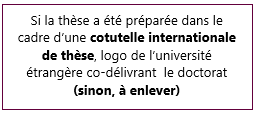
\includegraphics[scale=1]{logo2.png}

%*****************************************************
%******************** TITRE **************************
%*****************************************************

\flushright
\vspace{10mm} % à régler éventuellement
\color{Prune}
\fontfamily{cmss}\fontseries{m}\fontsize{22}{26}\selectfont
  \Huge 

\normalsize
\color{black}
~\\
\Large{Sign Language synthesis by a decreasing granularity system from AZee} \\
\small{\textit{Synthèse de langue des signes par un système d'animation à granularité décroissante à partir d'AZee}} \\
%*****************************************************

\fontfamily{fvs}\fontseries{m}\fontsize{8}{12}\selectfont

\vspace{1.5cm}

\normalsize
\textbf{Thèse de doctorat de l'université Paris-Saclay} \\

\vspace{6mm}

\small École doctorale n°580 : sciences et technologies de l’information et de la communication (STIC)\\
\small Spécialité de doctorat: informatique\\
\small Graduate School : Informatique et sciences du numérique, Référent : Faculté des sciences d’Orsay \\
\vspace{6mm}

\footnotesize Thèse préparée dans l'unité(s) de recherche \textbf{LISN} (Université Paris-Saclay, CNRS), sous la direction de \textbf{Michael FILHOL}, Chargé de recherche CNRS \\
\vspace{15mm}

\textbf{Thèse soutenue à Paris-Saclay, le JJ mois AAAA, par}\\
\bigskip
\Large {\color{Prune} \textbf{Paritosh SHARMA}} % Changer le Prénom et le NOM

%************************************
\vspace{\fill} % ALIGNER LE TABLEAU EN BAS DE PAGE
%************************************

\bigskip

\flushleft
\small {\color{Prune} \textbf{Composition du jury}}\\
{\color{Prune} \scriptsize {Membres du jury avec voix délibérative}} \\
\vspace{2mm}
\scriptsize
\begin{tabular}{|p{7cm}l}
\arrayrulecolor{Prune}
\textbf{Nicolas SABOURET} & Président\\ 
Professeur, Université Paris-Saclay \\
\textbf{John McDonald} &  Rapporteur \& Examinateur \\ 
Associate Professor, DePaul University \\ 
\textbf{Ludovic Hoyet} &  Rapporteur \& Examinateur \\ 
Chargé de recherche, INRIA \& Université de Rennes \\ 
\textbf{Catherine Pelachaud} &  Examinatrice \\ 
Directrice de recherche, CNRS - ISIR \& Sorbonne University \\ 
\textbf{Hui-Yin Wu} &  Examinateur ou Examinatrice \\ 
Chargé de recherche, Inria \& Université Côte d'Azur \\ 
 

\end{tabular} 

\end{titlepage}


% page des résumés à garder en 2ème page. Si les résumés sont trop longs pour tenir sur une seule et même page, on peut mettre un résumé par page
\thispagestyle{empty}
\newgeometry{top=1.5cm, bottom=1.25cm, left=2cm, right=2cm}
\fontfamily{rm}\selectfont

\lhead{}
\rhead{}
\rfoot{}
\cfoot{}
\lfoot{}

\noindent 
%*****************************************************
%***** LOGO DE L'ED À CHANGER IMPÉRATIVEMENT *********
%*****************************************************

\includegraphics[height=2.45cm]{logo_ups_STIC.png}
\vspace{1cm}
%*****************************************************
\fontfamily{cmss}\fontseries{m}\selectfont

\small

\begin{mdframed}[linecolor=Prune,linewidth=1]

\textbf{Titre:} Synthèse de langue des signes par un système d'animation à granularité décroissante à partir d'AZee

\noindent \textbf{Mots clés:} Animation Graphique, Signeur Virtuel, Langue des Signes

\vspace{-.5cm}
\begin{multicols}{2}
\noindent \textbf{Résumé:}

Les récents progrès dans la synthèse de la langue des signes ont permis de rapprocher ce domaine de la génération d'une langue des signes plus naturelle et expressive, mais des défis persistent. Les modèles actuels se concentrent souvent sur la synthèse au niveau des mots, ce qui peut entraîner une production manquant de fluidité et de naturel. Un des principaux défis de la synthèse de la langue des signes est de capturer les différentes granularités, allant des gestes larges aux mouvements subtils qui véhiculent des significations spécifiques. Pour surmonter cet obstacle, nous proposons un nouveau système de granularité décroissante basé sur le modèle AZee, qui organise la langue des signes en niveaux hiérarchiques, du plus grossier au plus fin.

Dans cette thèse, nous explorons l'application de ce système de granularité décroissante à la synthèse de la langue des signes. Notre objectif principal est de développer un système autonome capable de générer des séquences de langue des signes fluides et naturelles, adaptables à divers contextes et besoins des utilisateurs. Contrairement aux méthodes conventionnelles reposant sur des gestes prédéfinis et statiques, notre approche ajuste dynamiquement le niveau de granularité pendant la synthèse, assurant ainsi que la langue des signes générée soit à la fois contextuellement appropriée et expressive.

Tout au long de nos travaux, nous cherchons à approfondir la compréhension et l'application du formalisme AZee dans la synthèse de la langue des signes. Nous évaluons l'efficacité de notre approche en la comparant à d'autres méthodes existantes de synthèse de la langue des signes. Nos résultats montrent qu'un système de granularité décroissante peut grandement améliorer la naturalité et l'expressivité de la langue des signes synthétisée, ouvrant une voie prometteuse pour les recherches futures dans ce domaine.
\end{multicols}

\end{mdframed}

\newpage

\vspace{8mm}

\begin{mdframed}[linecolor=Prune,linewidth=1]

\textbf{Title:} Sign Language Synthesis by a Decreasing Granularity System from AZee

\noindent \textbf{Keywords:} Computer animation, Signing Avatars, Sign Language

\begin{multicols}{2}
\noindent \textbf{Abstract:}

Recent developments in sign language synthesis have brought the field closer to generating natural and expressive sign language, yet challenges remain. Current models often focus on word-level synthesis, resulting in output that can lack fluidity and naturalness. A major obstacle in sign language synthesis is the need to capture the varying granularities of sign language, ranging from broad gestures to subtle movements that convey specific meanings. To overcome this, we propose a novel decreasing granularity system based on the AZee model, which organizes sign language into hierarchical levels of granularity, from coarse to fine.

In this thesis, we investigate the application of this decreasing granularity system to sign language synthesis. Our primary objective is to develop an autonomous system capable of generating fluid and natural sign language sequences that are adaptable to different contexts and user needs. Unlike conventional approaches that rely on static, predefined gestures, our method dynamically adjusts the level of granularity during synthesis, ensuring that the generated sign language is both contextually appropriate and expressive.

Throughout our research, we focus on deepening the understanding and utility of the AZee formalism in sign language synthesis. We evaluate the effectiveness of our approach by comparing it with other existing means to synthesize Sign Language. Our findings demonstrate that a decreasing granularity system can greatly enhance the naturalness and expressiveness of synthesized sign language, presenting a promising avenue for future research in this area.

\end{multicols}
\end{mdframed}

\titleformat{\chapter}[display]
{\normalfont\huge\bfseries\color{black}} % Formatting for chapter title
{\chaptertitlename\ \thechapter} % "Chapter" followed by chapter number
{20pt} % Space between "Chapter" and chapter number
{\Huge} % Formatting for chapter title
[\vspace{2ex}] % Additional space after chapter title

\titlespacing*{\chapter}{0pt}{50pt}{40pt} % Adjusting spacing around chapter title

\titleformat{\section}[hang]{\bfseries\normalsize}{\thesection\ .}{0.5pt}
{\vspace{0.1ex}
}
[\vspace{0.1ex}]
\titlespacing{\section}{1.5pc}{4ex plus .1ex minus .2ex}{.8pc}

\titleformat{\subsection}[hang]{\bfseries\small}{\thesubsection\ .}{1pt}
{\vspace{0.1ex}
}
[\vspace{0.1ex}]
\titlespacing{\subsection}{3pc}{2ex plus .1ex minus .2ex}{.1pc}

\newpage
\thispagestyle{empty}
\vspace*{\fill}
\begin{center}
    \textit{"The only true wisdom is in knowing you know nothing."}\\
    --- \textbf{Socrates}
\end{center}
\vspace*{\fill}
\newpage

\subfile{acknowledgements/acknowledgements.tex}

\subfile{resume/resume.tex}

\newgeometry{top=4cm, bottom=4cm, left=2cm, right=2cm}

\newpage
\tableofcontents
\newpage
\listoffigures
\newpage
\listoftables
\newpage
\newglossaryentry{constraint}{
    name=constraint,
    description={todo}
}

\newglossaryentry{transpath}{
    name=transpath,
    description={todo}
}

\newglossaryentry{hold}{
    name=hold,
    description={todo}
}
\printglossaries
\newpage

\newgeometry{top=4cm, bottom=4cm, left=4cm, right=4cm}

\subfile{chapters/introduction/introduction.tex}
\subfile{chapters/background_work/background_work.tex}
\subfile{chapters/rigging_layers/rigging_layers.tex}
\subfile{chapters/multi_track/multi_track.tex}
\subfile{chapters/facial_expressions/facial_expressions.tex}
\subfile{chapters/intermediate_blocks/intermediate_blocks.tex}
\subfile{chapters/motion_matching/motion_matching.tex}
\subfile{chapters/conclusion/conclusion.tex}

\newgeometry{top=4cm, bottom=4cm, left=4cm, right=4cm}

\subfile{annex/annex.tex}

\bibliographystyle{apacite}
\bibliography{main}

\end{document}